\part{Fourier解析}
		\chapter{Fourier級数展開}
			\section{基底関数}
				Fourier級数展開の基底関数はFourier変換やDFTのものと違って正規化されていないため、美しさに欠ける。
				\par
				$d\in\naturalNumbers,\;W_l>0\;(l=1,2,,\cdots,d),\;\bm{k}\in\integers^d$とする。
				次式で定義される、$\bm{x}\in\realNumbers^d$に関する連続座標信号を、区間$\prod_{l=1}^d [-W_l,W_l]$に於ける第$\bm{k}$基底関数という。
				\[ W(\bm{k},\bm{x}) \coloneqq \exp i\sum_{l=1}^d k_l\frac{x_l}{W_l}\pi \]

			\section{Fourier係数}
				$d\in\naturalNumbers,\;W_l>0\;(l=1,2,,\cdots,d),\;\Omega\coloneqq\prod_{l=1}^d [-W_l,W_l],\;\bm{k}\in\integers^d$とする。
				$f:\bm{x}\in\realNumbers \mapsto f(\bm{x})\in\realNumbers$を、第$l$座標に関して周期が$2W_l$であるような周期関数とする。
				次式で定義する、$\bm{k}$に関する離散座標信号を$f$の第$\bm{k}$ Fourier係数という。
				\[ c(f,\bm{k}) \coloneqq \left(\prod_{l=1}^d 2W_l\right)^{-1}\integ{\Omega}{}{\conj{W(\bm{k},\bm{x})}f(\bm{x})}{\bm{x}} \]

		\chapter{Fourier変換}
			\section{基底関数}
				$d\in\naturalNumbers,\;\bm{x},\bm{\omega}\in\realNumbers^d$とする。
				次のものを$d$次元Fourier変換に於ける基底関数という。
				\[ W(\bm{\omega},\bm{x}) \coloneqq (2\pi)^{-d/2}\exp i\bm{\omega}^\top\bm{x} \]

			\section{Fourier変換の定義}
				$d\in\naturalNumbers,\;\bm{\omega}\in\realNumbers^d$とする。
				$f:\realNumbers^d\to\complexNumbers$に対して、次式で定義される、$\bm{\omega}$に関する連続座標信号を$f$のFourier変換という。
				\[ \mathcal{F}(f,\bm{\omega}) \coloneqq \integ{\realNumbers^d}{}{\conj{W(\bm{\omega},\bm{x})}f(\bm{x})}{\bm{x}} = (2\pi)^{-d/2} \integ{\realNumbers^d}{}{\exp (-i\bm{\omega}^\top\bm{x})f(\bm{x})}{\bm{x}} \]

		\chapter{離散時間Fourier変換(DTFT)}
			\section{直観的な説明}
				離散時間Fourier変換(Discrete Time Fourier Transform; DTFT)とは、直観的には、離散座標信号を、連続的な周波数をもつ無数の離散時間信号の重ね合わせとして表現するものである。
			\section{定義}
				$d\in\naturalNumbers$とする。
				$f:\integers^d\to\complexNumbers$に対して、次式で定義される、$\bm{\omega}\in\realNumbers^d$に関する連続座標信号を$f$の離散時間Fourier変換という。
				\[ \text{DTFT}(f,\bm{\omega}) \coloneqq \sum_{\bm{n}\in\integers^d} f(\bm{n})\exp(-i\bm{\omega}^\top\bm{n}) \]
				DTFTは周期関数であり、その周期は$(2\pi,2\pi,\dotsc,2\pi)$である。
				\subsection{呼称について}
					本書では関数の引数を時間や周波数に限定せず、より一般に座標と呼ぶ姿勢をとっている。
					しかしDTFTは電気・電子系の信号処理の分野で発展したため、離散``時間''という呼称が浸透しており、これに敢えて逆らって離散``座標''と呼ぶのは本書と工学応用の相性を悪くするだけで無益である。
					そこで、DTFTのような、歴史的な理由で呼称が定着しているものについては慣例に従うことにする。
			\section{連続座標信号との関係}
				連続座標信号$f_\text{c}:\realNumbers^d\to\complexNumbers$をサンプリング周期$\bm{T}_\text{s} \coloneqq [T_{\text{s},1}, T_{\text{s},2}, \dotsc, T_{\text{s},d}]^\top\in\realNumbers^d$すなわち周波数$\bm{f}_\text{s} \coloneqq [f_{\text{s},1}, f_{\text{s},2}, \dotsc, f_{\text{s},d}]^\top \coloneqq [1/T_{\text{s},1}, 1/T_{\text{s},2}, \dotsc, 1/T_{\text{s},d}]^\top\in\realNumbers^d$でサンプリングした離散座標信号を$f_\text{d}: \bm{n}\in\integers^d\mapsto f_\text{c}(\bm{T}^\top\bm{n})$とする。
				$f_\text{d}$のDTFTに於ける多次元の角周波数$\bm{\omega}$を周波数$\bm{f}$を用いて$\bm{\omega} \coloneqq 2\pi\bm{f}$と表す。
				\par
				$\bm{n}$の第$k$要素$n_k$が1だけ変化すると、元の連続座標信号の対応する座標は$T_k$だけ変化し、DTFTのカーネル関数$\exp(i\bm{\omega}^\top\bm{n})$の偏角は$\omega_k = 2\pi f_k$だけ変化する。
				つまりDTFTの定義域に於ける周波数$\bm{f}$の第$k$成分に対応する元の連続座標信号の周波数の第$k$成分は$\frac{1}{2\pi}\frac{\omega_k}{T_{\text{s},k}} = f_k f_{\text{s}, k}$である。
				ベクトル的に書けば、DTFTの定義域に於ける周波数$\bm{f}$に対応する元の連続座標信号の周波数は
				\[ \frac{1}{2\pi} \left(\nabla_\bm{n} \bm{\omega}^\top\bm{n}\right) \oslash \left(\nabla_\bm{n} \bm{T}_\text{s}^\top\bm{n}\right) = \bm{f} \odot \bm{f}_\text{s} \]
				ここに$\oslash, \odot$はそれぞれHadamard商, Hadamard積の演算子である。
				\par
				DTFTの定義で述べたように、DTFTは周期が$(2\pi,2\pi,\dotsc,2\pi)$であるから、一意に区別できる角周波数は$-\bm{\pi} \leq \bm{\omega} < \bm{\pi}$、つまり一意に区別できる周波数は$-\bm{1}/2 \leq \bm{f} < \bm{1}/2$である。
				この事実と、先程述べたDTFTと元の連続座標信号との周波数の関係から、DTFTに於いて一意に区別できる周波数に対応する元の連続座標信号の周波数$\tilde{\bm{f}}$は$-\bm{f}_\text{s}/2 \leq \tilde{\bm{f}} < \bm{f}_\text{s}/2$である。
			\section{逆離散時間Fourier変換(IDTFT)}
				$d\in\naturalNumbers, \Omega := [-\pi,\pi)^d$とする。
				$F:\realNumbers^d\to\complexNumbers$に対して、次式で定義される、$\bm{n}\in\integers^d$に関する離散座標信号を$F$の逆離散時間Fourier変換(Inverse DTFT; IDTFT)という。
				\[ \text{IDTFT}(F,\bm{n}) \coloneqq \frac{1}{(2\pi)^d}\integ{\Omega}{}{F(\bm{\omega})\exp(i\bm{\bm{\omega}}^\top\bm{n})}{\bm{\omega}} \]
				\subsection{IDTFTがDTFTの逆変換であること}
					厳密な導出はここでは述べないが、$\sum_{\bm{n}\in\integers^d} f(\bm{n})$が絶対収束する場合は$\text{IDTFT}(\text{DTFT}(f,\bm{\omega}),\bm{n}) = f(\bm{n})$となることを簡単に証明できる。
					$\sum$と$\int$の順序交換が簡単に行えるからである。
			\section{積と畳み込みとの関係}
				\subsection{時間領域, 周波数領域の畳み込みの定義}
					$d\in\naturalNumbers, \Omega := [-\pi,\pi)^d$とする。
					時間領域の畳み込みを次で定義する:
					\par
					$f,g:\integers^d\to\complexNumbers$に対してその畳み込み$f*g$を次式で定義する。
					\[ (f*g)(\bm{n}) := \sum_{\bm{m}\in\integers} f(\bm{m})g(\bm{n}-\bm{m}) \]
					周波数領域の畳み込みを次で定義する:
					\par
					$F,G:\realNumbers^d\to\complexNumbers$に対してその畳み込み$F*G$を次式で定義する。
					\[ (F*G)(\bm{\omega}) := \frac{1}{(2\pi)^d}\integ{\Omega}{}{F(\tilde{\bm{\omega}})G(\bm{\omega}-\tilde{\bm{\omega}})}{\tilde{\bm{\omega}}} \]
				\subsection{積のDTFT}
					$d\in\naturalNumbers,\;\Omega := [-\pi,\pi)^d,\;\bm{\omega}\in\realNumbers^d$とする。
					$f,g:\integers^d\to\complexNumbers$に対してそのDTFTを$F(\bm{\omega}),G(\bm{\omega})$とする。
					$f,g$の積のDTFTは次式で求まる。
					\begin{align*}
						\text{DTFT}(fg,\bm{\omega}) &= \sum_{n\in\integers} f(\bm{n})g(\bm{n})\exp(-i\bm{\omega}^\top\bm{n}) = \sum_{n\in\integers} \text{IDTFT}(F,\bm{n}) g(\bm{n})\exp(-i\bm{\omega}^\top\bm{n}) \\
						&= \sum_{n\in\integers} \left(\frac{1}{(2\pi)^d}\integ{\Omega}{}{F(\tilde{\bm{\omega}})e^{i\tilde{\bm{\omega}}^\top\bm{n}}}{\tilde{\bm{\omega}}}\right) g(\bm{n})\exp(-i\bm{\omega}^\top\bm{n}) \\
						&= \frac{1}{(2\pi)^d}\integ{\Omega}{}{F(\tilde{\bm{\omega}})\left(\sum_{n\in\integers} g(\bm{n})e^{-i(\bm{\omega}-\tilde{\bm{\omega}})^\top\bm{n}}\right)}{\tilde{\bm{\omega}}} \\
						&= \frac{1}{(2\pi)^d}\integ{\Omega}{}{F(\tilde{\bm{\omega}})G(\bm{\omega}-\tilde{\bm{\omega}})}{\tilde{\bm{\omega}}} = (F*G)(\omega)
					\end{align*}
				\subsection{畳み込みのDTFT}
				\subsection{積のIDTFT}
				\subsection{畳み込みのIDTFT}
			\section{定数関数1のDTFT}
				\label{定数関数1のDTFT}
				簡単のため1次元の場合について考察する。
				工学系の学生を対象とする講義では、$\text{DTFT}(1,\omega) = 2\pi\sum_{m\in\integers}\delta(\omega-2m\pi)$($\delta$はDiracのデルタ関数)を詳細を割愛して結果として受け入れさせる場合が多いと思う。
				$\text{IDTFT}\left(2\pi\sum_{m\in\integers}\delta(\omega-2m\pi),x\right)=1$の確認は簡単であり、DTFTの可逆性から$\text{DTFT}(1,\omega) = 2\pi\sum_{m\in\integers}\delta(\omega-2m\pi)$を受け入れる説明がなされると思う。
				\par
				ここではDirichlet積分を用いて$\text{DTFT}(1,\omega) = 2\pi\sum_{m\in\integers}\delta(\omega-2m\pi)$を直接的に考察してみる。
				DTFTの定義から次式が成り立つ。
				\[
					\text{DTFT}(1,\omega) = \lim_{N\to\infty} \sum_{m=-N}^N e^{i\omega m} = \frac{\sin(N+1/2)\omega}{\sin(\omega/2)}
				\]
				最右辺は等比数列の和の公式を用いた後、分母と分子に$e^{-i\omega/2}$を掛けて整理すると得られる。
				これが$N\to\infty$で$2\pi\sum_{m\in\integers}\delta(\omega-2m\pi)$として振る舞うことを確かめる。
				$2\pi$周期性については明らかだから、$[-\pi,\pi)$の範囲で$\delta(\omega)$として振る舞うことを確かめれば十分である。
				示すべきことは次の通りである。
				\begin{shadebox}
					$d\in\naturalNumbers$とする。
					区間$\Omega \subseteq [-\pi,\pi)$上で連続な関数$f:\Omega\to\complexNumbers^d$を考える。
					$h>0$を$[-h,h) \subseteq \Omega$となるように任意にとる。
					このとき次式が成り立つ。
					\[
						\lim_{N\to\infty} \integ{-h}{h}{\frac{\sin(N+1/2)x}{\sin(x/2)} f(x)}{x} = 2\pi f(0)
					\]
				\end{shadebox}
				\begin{proof}
					\quad\par
					極限をとる前の積分を$I_N$とおく。
					$y = x/2$と変数変換すると次式を得る。
					\[
						I_N = 2\integ{-h/2}{h/2}{\frac{\sin(2N+1)y}{\sin y}f(2y)}{y} = 2\integ{-h/2}{h/2}{\frac{\sin(2N+1)y}{y}\frac{y}{\sin y}f(2y)}{y}
					\]
					後に現れるDirichlet積分の性質から$N\to\infty$で積分の主要部分が$x=0$近傍に集中することがこの時点で推察できる。
					そこで、十分に小さい正数$d'$を$0<d'<h/2$となるようにとり、積分区間を$[-h/2,-d']\cup[-d',d']\cup[d',h/2]$と分割する。
					\par
					$[-h/2,-d'], [d',h/2]$に於いて$f(2y)/\sin y$は一様連続であるので$N\to\infty$でこの2つの区間に於ける$(f(2y)\sin(2N+1)y)/\sin y$の積分は0に収束する。
					証明の方針としては、$\sin(2N+1)y$の符号が変化する点で積分区間を細分し、格区間内で$f(2y)/\sin y$を定数で近似して全体の積分を近似すると、一様連続性から近似値と真の積分の差が0に収束し、かつ近似値が0に収束する。
					\par
					つまり任意に小さい$\varepsilon>0$に対して、$d'$に依存して決まる十分大きい自然数$N_1$が存在して次式が成り立つ。
					\[
						N\geq N_1 \Rightarrow \abs{2\integ{[-h/2,-d']\cup[d',h/2]}{}{\frac{\sin(2N+1)y}{\sin y}f(2y)}{y}}<\varepsilon
					\]
					\par
					次に$[-d',d']$に於ける積分を評価する。
					$y\to 0$で$y/\sin y\to 1,\;f(2y)\to f(0)$であるから、$d'$を十分小さくとりなおすことで$|f(2y)y/\sin y - f(0)| < \varepsilon$となり次式が成り立つ。
					\[
						\abs{2\integ{-d'}{d'}{\frac{\sin(2N+1)y}{y}\frac{y}{\sin y}f(2y)}{y} - 2f(0)\integ{-d'}{d'}{\frac{\sin(2N+1)y}{y}}{y}} < 2\varepsilon\abs{\integ{-d'}{d'}{\frac{\sin(2N+1)y}{y}}{y}}
					\]
					最後にDirichlet積分を用いて$(\sin(2N+1)y)/\sin y$の積分を評価する。
					\[
						\integ{-d'}{d'}{\frac{\sin(2N+1)y}{y}}{y} = 2\integ{0}{d'}{\frac{\sin(2N+1)y}{y}}{y} = 2\integ{0}{(2n+1)d'}{\frac{\sin z}{z}}{z} \to \pi \text{ as } n\to\infty
					\]
					すなわち$d'$に依存して決まる十分大きい自然数$N_2$が存在して次式が成り立つ。
					\[ N\geq N_1 \Rightarrow \abs{\integ{-d'}{d'}{\frac{\sin(2N+1)y}{y}}{y} - \pi} < \varepsilon \]
					以上より、$d'>0$を十分に小さくとり、$N\geq\max(N_1,N_2)$とすれば次式が成り立つ。
					\begin{align*}
						|I_N - 2\pi f(0)| &= \left|\underbrace{\left(2f(0)\integ{-d'}{d'}{\frac{\sin(2N+1)y}{y}}{y} - 2\pi f(0)\right)}_{(1)} \right. \\
						&\phantom{=} \left.+ \underbrace{\left(2\integ{-d'}{d'}{\frac{\sin(2N+1)y}{y}\frac{y}{\sin y}f(2y)}{y} - 2f(0)\integ{-d'}{d'}{\frac{\sin(2N+1)y}{y}}{y}\right)}_{(2)} \right. \\
						&\phantom{=} \left.+ \underbrace{2\integ{[-h/2,-d']\cup[d',h/2]}{}{\frac{\sin(2N+1)y}{\sin y}f(2y)}{y}}_{(3)}\right| \\
						&\leq |(1)| + |(2)| + |(3)| < 2f(0)\varepsilon + 2\varepsilon(\pi+\varepsilon) + \varepsilon
					\end{align*}
				\end{proof}
			\section{単一周波数波のDTFTの導出}
				$\sin\omega_0 n,\cos\omega_0 n\;(\omega_0\in\realNumbers, n\in\integers)$のDTFTは\ref{定数関数1のDTFT}の結果を用いて次のようにして得られる。
				\begin{align*}
					\begin{split}
						\text{DTFT}(\sin\omega_0 n, \omega) &= \sum_{n=-\infty}^\infty \frac{e^{i\omega_0 n} - e^{-i\omega_0 n}}{2i}e^{-i\omega n} = \frac{1}{2i}\sum_{n=-\infty}^\infty \left(e^{-i(\omega-\omega_0) n} - e^{-i(\omega+\omega_0) n}\right) \\
						&= -i\pi\sum_{m\in\integers}\bigl(\delta(\omega-\omega_0-2m\pi) - \delta(\omega+\omega_0-2m\pi)\bigr) \\
						&= i\pi\sum_{m\in\integers}\bigl(\delta(\omega+\omega_0-2m\pi) - \delta(\omega-\omega_0-2m\pi)\bigr)
					\end{split} \\
					\begin{split}
						\text{DTFT}(\cos\omega_0 n, \omega) &= \sum_{n=-\infty}^\infty \frac{e^{i\omega_0 n} + e^{-i\omega_0 n}}{2}e^{-i\omega n} = \frac{1}{2}\sum_{n=-\infty}^\infty \left(e^{-i(\omega-\omega_0) n} + e^{-i(\omega+\omega_0) n}\right) \\
						&= \pi\sum_{m\in\integers}\bigl(\delta(\omega-\omega_0-2m\pi) + \delta(\omega+\omega_0-2m\pi)\bigr)
					\end{split}
				\end{align*}
			\section{システムの伝達関数と正弦波入力の関係}
		\chapter{離散Fourier変換(DFT)}
			\section{基底}
				$d\in\naturalNumbers,\;N_l\in\naturalNumbers\;(l=1,2,\cdots,d),\;\bm{k},\bm{n}\in\integers^d$とする。
				次式で定義される、$\bm{n}$に関する離散座標信号を$d$次元DFTの第$\bm{k}$基底ベクトルという。
				\[ W(\bm{k},\bm{n}) \coloneqq \left(\prod_{l=1}^d N_l\right)^{-1/2} \exp i\left(\sum_{l=1}^d \frac{k_l n_l}{N_l}2\pi\right)\]

			\section{DFTの定義}
				\label{DFTの定義}
				$d\in\naturalNumbers,\;N_l\in\naturalNumbers\;(l=1,2,\cdots,d),\;\bm{k}\in\integers^d$とする。
				$\Omega \coloneqq \{0,1,\cdots,N_1-1\}\times\{0,1,\cdots,N_2-1\}\times\cdots\times\{0,1,\cdots,N_d-1\}$とする。
				$f$を周期が$(N_1,N_2,\cdots,N_d)$であるような離散座標信号$f: \integers^d\to\complexNumbers;\;\bm{n} = [n_1,n_2,\cdots,n_d]^\top \mapsto f(\bm{n})$とするとき、次式で定義される、$\bm{k}$に関する離散座標信号を$f$の離散Fourier変換(Discrete Fourier Transform; DFT)という。
				\[ \text{DFT}(f,\bm{k}) \coloneqq \sum_{\bm{n}\in\Omega} \conj{W(\bm{k},\bm{n})} f(\bm{n}) \]

			\section{Hermiteな離散時間信号のDFTは実数である}
				\label{Hermiteな離散時間信号のDFTは実数である}
				\begin{shadebox}
					$d,N_l,\bm{k},\Omega,f$の定義は\ref{DFTの定義}と同じものとする。
					$f$にさらにHermite性: $\conj{f(\bm{n})} = f(-\bm{n})$を要請するとき、$\text{DFT}(f,\bm{k})$は実数となる。
				\end{shadebox}
				\begin{proof}
					\begin{align*}
						2\Im{\text{DFT}(f,\bm{k})} &= \text{DFT}(f,\bm{k}) - \conj{\text{DFT}(f,\bm{k})} \\
						&= \sum_{\bm{n}\in\Omega} \conj{W(\bm{k},\bm{n})}f(\bm{n}) - \sum_{\bm{n} \in \Omega}W(\bm{k},\bm{n})\conj{f(\bm{n})}
					\end{align*}
					ここで$\bm{n}_\text{M} \coloneqq [N_1,\cdots,N_d]^\top$とすると、
					\[ \conj{W(\bm{k},\bm{n})} = W(\bm{k},-\bm{n}) = W(\bm{k},\bm{n}_\text{M}-\bm{n}) \]
					また、$f$のHermite性の仮定より
					\[ \conj{f(\bm{n})} = f(-\bm{n}) = f(\bm{n}_\text{M}-\bm{n}) \]
					以上より
					\begin{align*}
						2\Im{\text{DFT}(f,\bm{k})} &= \sum_{\bm{n}\in\Omega} W(\bm{k},\bm{n}_\text{M}-\bm{n})f(\bm{n}) - \sum_{\bm{n} \in \Omega}W(\bm{k},\bm{n})f(\bm{n}_\text{M}-\bm{n}) \\
						&= \sum_{\bm{n}\in\Omega} W(\bm{k},\bm{n}_\text{M}-\bm{n})f(\bm{n}) - \sum_{\bm{n}\in\Omega} W(\bm{k},\bm{n}_\text{M}-\bm{n})f(\bm{n}) \\
						&\phantom{=} (\{(\bm{n}, \bm{n}_\text{M}-\bm{n}) | \bm{n}\in\Omega\} = \{(\bm{n}_\text{M}-\bm{n}), \bm{n} | \bm{n}\in\Omega\}\text{を用いた}) \\
						&= 0
					\end{align*}
				\end{proof}

			\subsection{系: Hermiteな離散時間信号のIDFTは実数である}
				\ref{Hermiteな離散時間信号のDFTは実数である}と同様にして示せる。

			\section{巡回畳み込みのDFTはDFTの積に比例する}
				\begin{shadebox}
					$d,N_l,\bm{k},\Omega$の定義は\ref{DFTの定義}と同じものとする。
					$f,g$を周期が$(N_1,N_2,\cdots,N_d)$であるような離散座標信号$f,g: \integers^d\to\complexNumbers;\;\bm{n} = [n_1,n_2,\cdots,n_d]^\top \mapsto f(\bm{n}),g(\bm{n})$とするとき、次が成り立つ。
					\[ \text{DFT}\left(\cycConv{f}{g},\bm{k}\right) = \left(\prod_{l=1}^d N_l\right)^{1/2}\text{DFT}(f,\bm{k})\text{DFT}(g,\bm{k}) \]
				\end{shadebox}
				\begin{proof}
					\quad\par
					$\bm{N} \coloneqq [N_1,\cdots,N_d]^\top$とする。
					\begin{align*}
						\text{DFT}\left(\cycConv{f}{g},\bm{k}\right) &= \sum_{\bm{n}\in\Omega}\conj{W(\bm{k},\bm{n})} \left(\cycConv{f}{g}\right)(\bm{n}) = \sum_{\bm{n}\in\Omega}\conj{W(\bm{k},\bm{n})} \sum_{\bm{m}\in\Omega} f(\bm{m})g((\bm{n}-\bm{m})\%\bm{N}) \\
						&= \sum_{\bm{m}\in\Omega} f(\bm{m}) \sum_{\bm{n}\in\Omega} \conj{W(\bm{k},\bm{n})}g((\bm{n}-\bm{m})\%\bm{N}) \\
						&= \sum_{\bm{m}\in\Omega} f(\bm{m}) \sum_{\bm{n}\in\Omega} \left(\prod_{l=1}^d N_l\right)^{1/2} \conj{W(\bm{k},\bm{m})} \conj{W(\bm{k},\bm{n}-\bm{m})} g((\bm{n}-\bm{m})\%\bm{N}) \\
						&= \left(\prod_{l=1}^d N_l\right)^{1/2} \sum_{\bm{m}\in\Omega} \conj{W(\bm{k},\bm{m})}f(\bm{m}) \sum_{\bm{n}\in\Omega} \conj{W(\bm{k},(\bm{n}-\bm{m})\%\bm{N})} g((\bm{n}-\bm{m})\%\bm{N}) \\
						&= \left(\prod_{l=1}^d N_l\right)^{1/2} \sum_{\bm{m}\in\Omega} \conj{W(\bm{k},\bm{m})}f(\bm{m}) \sum_{\bm{n}\in\Omega} \conj{W(\bm{k},\bm{n})} g(\bm{n}) \\
						&= \left(\prod_{l=1}^d N_l\right)^{1/2}\text{DFT}(f,\bm{k})\text{DFT}(g,\bm{k})
					\end{align*}
				\end{proof}

			\section{GaussianノイズのDFT}
				\begin{shadebox}
					$F(n) \in \complexNumbers\;(n=0,1,\cdots,N-1)$は互いに独立で、複素正規分布$N(0,\sigma^2)$に従うとする$\left(\text{p}(f) = \frac{1}{2\pi\sigma^2}\exp\frac{-\Re{f}^2-\Im{f}^2}{2\sigma^2} = \frac{1}{2\pi\sigma^2}\exp\frac{-|f|^2}{2\sigma^2}\right)$。
					これのDFTを$G(k) = \text{DFT}(F,k)$とするとき、$G(k)\;(k=0,1,\cdots,N-1)$もまた互いに独立で、複素正規分布$N(0,\sigma^2)$に従う。
				\end{shadebox}
				\begin{proof}
					\[ P \in \complexNumbers^{N\times N},\; P_{k,n} \coloneqq W(k,n) \coloneqq \frac{1}{\sqrt{N}}\exp i\frac{kn}{N}2\pi\;(k,n \in \{0,1,\cdots,N-1\}) \]
					\[ \bm{F} \coloneqq [F(0), F(1), \cdots, F(N-1)]^\top,\;\bm{G} \coloneqq [G(0), G(1), \cdots, G(N-1)]^\top \]
					と定義すると
					\[ \bm{G} = P^*\bm{F} \]
					となる。
					\begin{align*}
						\Pr{\bm{G} = \bm{g} \in \complexNumbers^N} &= \Pr{P^*\bm{F} = \bm{g}} = \Pr{\bm{F} = P\bm{g}} \\
						&= \prod_{i=0}^{N-1}\frac{1}{2\pi\sigma^2} \exp\frac{-|(P\bm{g})[i]|^2}{2\sigma^2} = \left(\prod_{i=0}^{N-1}\frac{1}{2\pi\sigma^2}\right) \exp \sum_{i=0}^{N-1} \frac{-|(P\bm{g})[i]|^2}{2\sigma^2} \\
						&= \left(\prod_{i=0}^{N-1}\frac{1}{2\pi\sigma^2}\right) \exp \frac{-\norm{P\bm{g}}_2^2}{2\sigma^2} = \left(\prod_{i=0}^{N-1}\frac{1}{2\pi\sigma^2}\right) \exp \frac{-\norm{\bm{g}}_2^2}{2\sigma^2} \\
						&= \prod_{i=0}^{N-1}\frac{1}{2\pi\sigma^2} \exp \frac{-|g_i|^2}{2\sigma^2}
					\end{align*}
				\end{proof}

		\chapter{サンプリング定理}
			\begin{shadebox}
				$d\in\naturalNumbers,\;W_l>0\;(l=1,2,,\cdots,d),\;\Omega\coloneqq\prod_{l=1}^d [-W_l,W_l]$とする。
				$f:\realNumbers^d\to\realNumbers$のFourier変換$\mathcal{F}(f,\bm{\omega})$が存在してその台が$\Omega$に含まれるとき、次式が成り立つ。
				\[ f(\bm{x}) = \sum_{\bm{n}\in\naturalNumbers}f\left(\pi\frac{n_1}{W_1},\cdots,\pi\frac{n_d}{W_d}\right)\prod_{l=1}^d\sinc W_l\left(x_l + \pi\frac{n_l}{W_l}\right) \]
				つまり$f$の各点での評価値を沢山集めて$f$を任意の精度で近似できる。
				\par
				角周波数$W_l$のかわりに周波数$F_l=W_l/(2\pi)$を使うと上式は次式になる。
				\[ f(\bm{x}) = \sum_{\bm{n}\in\naturalNumbers}f\left(\frac{n_1}{2F_1},\cdots,\frac{n_d}{2F_d}\right)\prod_{l=1}^d\sinc 2\pi F_l\left(x_l + \frac{n_l}{2F_l}\right) \]
			\end{shadebox}
			\begin{proof}
				\quad\par
				$\mathcal{F}(f,\bm{\omega})$の台が超直方体$\Omega$に含まれるから$\mathcal{F}(f,\bm{\omega})$はFourier級数展開できる。
				第$\bm{n}$Fourier係数を$c(\mathcal{F}(f),\bm{n})$とすると
				\[ \mathcal{F}(f,\bm{\omega}) = \sum_{\bm{n}\in\naturalNumbers^d} c(\mathcal{F}(f),\bm{n}) \exp i\sum_{l=1}^d n_l\frac{\omega_l}{W_l}\pi \]
				となる。$c(\mathcal{F}(f),\bm{n})$は次式で求まる。
				\begin{align*}
					c(\mathcal{F}(f),\bm{n}) &= \left(\prod_{l=1}^d 2W_l\right)^{-1} \integ{\Omega}{}{\mathcal{F}(f,\bm{\xi}) \exp (-i)\sum_{l=1}^d n_l\frac{\xi_l}{W_l}\pi}{\bm{\xi}} \\
					&= (2\pi)^{d/2} \left(\prod_{l=1}^d 2W_l\right)^{-1} (2\pi)^{-d/2} \integ{\textcolor{darkpastelgreen}{\realNumbers^d}}{}{\mathcal{F}(f,\bm{\xi}) \exp i\sum_{l=1}^d \left(\frac{-n_l}{W_l}\pi\right)\xi_l}{\bm{\xi}} \\
					&= (2\pi)^{d/2} \left(\prod_{l=1}^d 2W_l\right)^{-1} \mathcal{F}^{-1}\left(\mathcal{F}(f),-\pi\bm{n}\oslash\bm{W}\right) \\
					&= (2\pi)^{d/2} \left(\prod_{l=1}^d 2W_l\right)^{-1} f\left(-\pi\bm{n}\oslash\bm{W}\right)
				\end{align*}
				$f$は$\mathcal{F}(f)$のFourier逆変換で次のようにして求まる。
				\begin{align*}
					f(\bm{x}) &= \mathcal{F}^{-1}\left(\mathcal{F}(f),\bm{x}\right) = (2\pi)^{-d/2} \integ{\realNumbers^d}{}{\mathcal{F}(f,\bm{\omega})\exp i\bm{\omega}^\top\bm{x}}{\bm{\omega}} = (2\pi)^{-d/2} \integ{\Omega}{}{\mathcal{F}(f,\bm{\omega})\exp i\bm{\omega}^\top\bm{x}}{\bm{\omega}} \\
					&= (2\pi)^{-d/2} \integ{\Omega}{}{\sum_{\bm{n}\in\naturalNumbers^d} c(\mathcal{F}(f),\bm{n}) \left(\exp i\sum_{l=1}^d n_l\frac{\omega_l}{W_l}\pi\right) \exp i\bm{\omega}^\top\bm{x}}{\bm{\omega}} \\
					&= (2\pi)^{-d/2} \sum_{\bm{n}\in\naturalNumbers^d} \integ{\Omega}{}{c(\mathcal{F}(f),\bm{n}) \exp i \bm{\omega}^\top\left(\bm{x} + \pi\bm{n}\oslash\bm{W}\right) }{\bm{\omega}} \\
					&= (2\pi)^{-d/2} \sum_{\bm{n}\in\naturalNumbers^d} \integ{\Omega}{}{(2\pi)^{d/2} \left(\prod_{l=1}^d 2W_l\right)^{-1} f\left(-\pi\bm{n}\oslash\bm{W}\right) \exp i \bm{\omega}^\top\left(\bm{x} + \pi\bm{n}\oslash\bm{W}\right) }{\bm{\omega}} \\
					&= \left(\prod_{l=1}^d 2W_l\right)^{-1} \sum_{\bm{n}\in\naturalNumbers^d} f\left(-\pi\bm{n}\oslash\bm{W}\right) \integ{\Omega}{}{\exp i \bm{\omega}^\top\left(\bm{x} + \pi\bm{n}\oslash\bm{W}\right) }{\bm{\omega}}
				\end{align*}
				ここで
				\begin{align*}
					\integ{\Omega}{}{\exp i \bm{\omega}^\top\left(\bm{x} + \pi\bm{n}\oslash\bm{W}\right) }{\bm{\omega}} &= \prod_{l=1}^d \integ{-W_l}{W_l}{\exp i\left(x_l + \pi\frac{n_l}{W_l}\right)\omega_l}{\omega_l} \\
					&= \prod_{l=1}^d \frac{1}{i\left(x_l + \pi\frac{n_l}{W_l}\right)}\left[\exp i\left(x_l + \pi\frac{n_l}{W_l}\right)W_l - \exp (-i)\left(x_l + \pi\frac{n_l}{W_l}\right)W_l\right] \\
					&= \prod_{l=1}^d 2W_l \frac{\sin \left(x_l + \pi\frac{n_l}{W_l}\right)W_l}{\left(x_l + \pi\frac{n_l}{W_l}\right)W_l} = \prod_{l=1}^d 2W_l \prod_{l=1}^d \sinc W_l\left(x_l + \pi\frac{n_l}{W_l}\right)
				\end{align*}
				であるから
				\begin{align*}
					f(\bm{x}) &= \sum_{\bm{n}\in\naturalNumbers^d} f\left(-\pi\bm{n}\oslash\bm{W}\right) \prod_{l=1}^d 2W_l \sinc \left(x_l + \pi\frac{n_l}{W_l}\right)W_l = \sum_{\bm{n}\in\naturalNumbers^d} f\left(\pi\bm{n}\oslash\bm{W}\right) \prod_{l=1}^d \sinc W_l\left(x_l - \pi\frac{n_l}{W_l}\right) \\
					&= \sum_{\bm{n}\in\naturalNumbers^d} f\left(\pi\frac{n_1}{W_1},\cdots,\pi\frac{n_d}{W_d}\right) \prod_{l=1}^d \sinc W_l\left(x_l - \pi\frac{n_l}{W_l}\right)
				\end{align*}
			\end{proof}
		\chapter{高速Fourier変換(FFT)}
			\section{長さが2のべき乗でない信号のDFTを長さが2のべき乗の信号のFFTに帰着する方法}
				$N$を$2$のべき乗でない自然数とする。
				長さ$N$の信号$x$のDFT
				\[ X(k) = \frac{1}{\sqrt{N}} \sum_{n=0}^{N-1} x(n)\exp \left(2\pi i\frac{-kn}{N}\right) \quad k=1,2,\cdots,N-1 \]
				を長さが$2$のべき乗である信号のFFTに帰着する方法を考える。
				$\forall a,b\in\mathbb{R},\;ab = \frac{a^2 + b^2 - (a-b)^2}{2}$を用いて上の式を次のように変形する。
				\begin{align*}
					\begin{aligned}
						X(k) &= \frac{1}{\sqrt{N}} \exp \left(\pi i\frac{-k^2}{N}\right) \sum_{n=0}^{N-1} x(n)\exp \left(\pi i\frac{-n^2}{N}\right) \exp \left(\pi i\frac{(k-n)^2}{N}\right) \\
						&= \frac{1}{\sqrt{N}} \exp \left(\pi i\frac{-k^2}{N}\right) \sum_{n=0}^{N-1} u(n)v(k-n) \\
						& \text{where} \quad u(n) \coloneqq x(n)\exp \left(\pi i\frac{-n^2}{N}\right),\;v(n) \coloneqq \exp \left(\pi i\frac{n^2}{N}\right)
					\end{aligned}
				\end{align*}
				\[ \therefore\; X(k)\sqrt{N} \exp \left(\pi i\frac{k^2}{N}\right) = (u*v)(k) \]
				$u*v$を、長さが$2$のべき乗の信号に対して使えるFFT, IFFTを用いて計算する。
				そのために長さが$2$のべき乗の信号同士の**巡回畳み込み**の中に$u*v$が部分的に現れるような状況を以下のようにして作り出す。
				\par
				$N_2 \coloneqq \min\{a|\exists b\in \mathbb{N}, a = 2^b \geq 2N\}$ とする。
				長さ$N_2$の信号$u_2,v_2$を以下のように定義する。
				\[
					u_2(n) \coloneqq \left\{
						\begin{aligned}
							u(n) &\quad (n \in [0,N-1]) \\
							0 &\quad (n \in [N,N_2-1])
						\end{aligned}
					\right.
				\]
				\[
					v_2(n) \coloneqq \left\{
						\begin{aligned}
							v(n) &\quad (n \in [0,N-1]) \\
							0 &\quad (n\in [N,N_2-N]) \\
							v(N_2-n) &\quad (n \in [N_2-N+1,N_2-1])
						\end{aligned}
					\right.
				\]
				$u_2$は$u$の後ろに$0$を並べて長さ$N_2$に拡張した信号である。
				$v_2$は長さ$N_2$の$0$が並んだ信号の前部を$v$で塗り替え、後部を$v$の第$1\sim N-1$要素をコピーして順番を逆にしたもので塗り替えた信号である。
				下の図は$u_2,v_2$を視覚的に表現したものである。
				\begin{figure}[H]
					\centering
					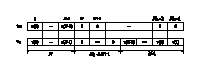
\includegraphics[keepaspectratio, scale=4]
					{parts/FourierAnalysis/imgs/FFT/arbitraryLengthFFT_to_powerOf2_FFT/u2,v2.eps}
					\caption{$u_2,v_2$の構造}
				\end{figure}
				このようにすると$u_2*v_2$の先頭$N$要素が$u*v$と一致する。
				\[ \text{FFT}(u_2*v_2) = \sqrt{N_2}\text{ FFT}(u_2) \text{ FFT}(v_2) \]
				より
				\[ \text{IFFT}(\sqrt{N_2}\text{ FFT}(u_2) \text{ FFT}(v_2)) \]
				により$u_2*v_2$を高速に計算し、結果の先頭$N$要素を切り出せば$u*v$を得る。
				得られた$u*v$の第$k$要素に$\frac{1}{\sqrt{N}} \exp \left(\pi i\frac{-k^2}{N}\right)$を掛ければ$x$のDFTが得られる。
				$v_2$のFFTや$\frac{1}{\sqrt{N}} \exp \left(\pi i\frac{-k^2}{N}\right) \;(k=0,1,\cdots,N-1)$は初回の計算結果を保存しておけば別の信号のDFTの計算で再利用できる。
